\section{3D-Modell}
\label{sec:3Dmodel}
Zur Veranschaulichung von verschiedenen Komponenten und mechanischen Ausführungen in verschiedenen Ansichten und Perspektiven, ist ein 3D-Modell besonders gut geeignet. Sämtliche 3D-gedruckten Konstruktionen werden mithilfe der \ac{CAD}-Anwendung \glqq Solidworks\grqq\ erstellt. Das Modellieren des Modellautos sowie die Zusammenfügung, Texturierung und Belichtung aller Komponenten, wird mit der freien Software \glqq Blender\grqq\ gemacht. Blender ermöglicht zum einen das Modellieren von komplexen Körpern und Figuren. Außerdem können diese mit einem benutzerdefinierten Material texturiert werden. Mit Hilfe der korrekten Belichtung können somit fotorealistische Grafiken erzeugt werden. Dazu wird mit einer virtuellen Kamera ein Ausschnitt des Modells gewählt, welcher anschließend in einer beliebigen Auflösung \glqq gerendert\grqq\ werden kann. Als \glqq Rendering\grqq\ wird die Erstellung einer Grafik aus Rohdaten, in diesem Fall also aus einem 3D-Modell, bezeichnet. Dabei werden unter anderem sämtliche Lichtreflexionen an den verschiedenen Materialien berechnet.
\begin{figure}[h]
\centering
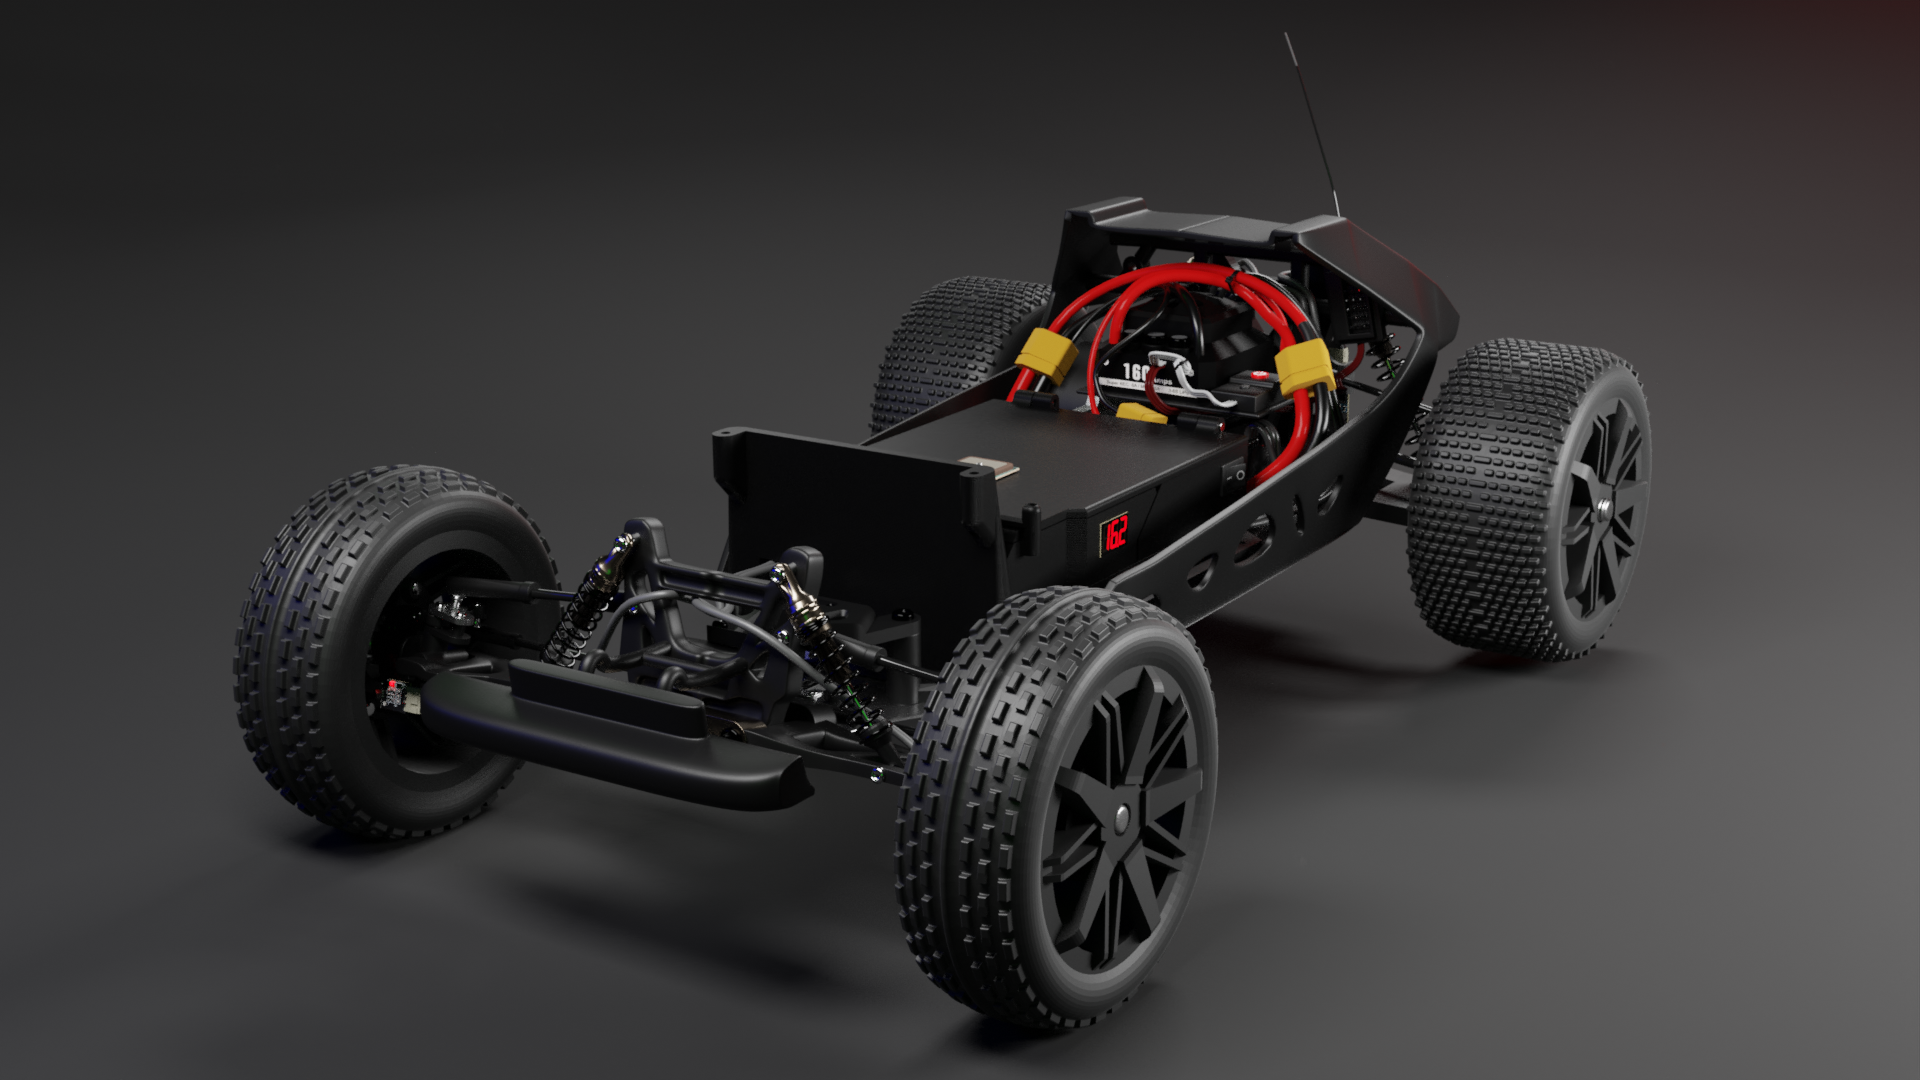
\includegraphics[scale=0.2]{3DModel_front.png}
\caption{\ac{3D}-Modell von vorne}
\label{fig:3DFront}
\end{figure}

\begin{figure}[h]
\centering
\includegraphics[scale=0.2]{3DModel_floor.png}
\caption{\ac{3D}-Modell auf Holzboden}
\label{fig:3DWood}
\end{figure}